\chapter{Experiments}
\label{chapter:experiments}
% \{for motivation, maybe consider the introduction \href{https://arxiv.org/pdf/1712.03346.pdf}{here}}

In chapter \ref{chapter:introduction} we asked how well good protein representations are achieved by machine learning models, how they can be implemented, what the advantages and disadvantages of global versus local representations are, and how the properties of the representation affect the performance on downstream tasks.

In order to find answers, we have carried out a number of experiments, applied to each model. There are broadly two experimental settings: (1) mutation effect prediction and (2) tasks assessing protein embeddings, otherwise known as TAPE \cite{rao2019evaluating}. The first setting evaluates the mutation effect prediction of the models, based on the learned distribution over proteins. This is of interest, as mutation effect prediction is tightly connected to the underlying evolutionary generating process, and what properties the mutated protein possesses. The second setting is a benchmark assessment of the performance of the protein representations on downstream tasks.

In this chapter we report how we did it and what the results were. In section \ref{sec:experimental_setup} the experimental settings are accounted for, including commonalities between the experiments such as what language framework we used to implement the models, and hardware used for training and testing. 

There are three conceptually different model architectures that we have tested. Each model architecture is described in chapter \ref{chapter:models} and has its own section here with implementation details, results and discussion.

% In section \ref{sec:unirep_experiment}, the UniRep model \cite{alley2019unified}. UniRep is a recurrent model, and can thus handle variable-length sequences, and can thus be trained on global protein databases. We explore the performance of a variant of the UniRep model on downstream tasks.

% In section \ref{sec:variational_autoencoders_experiement}, we explore the usefulness of the Variational Autoencoder on protein sequences. Specifically, we train a Variational Autoencoder model on sequences within single protein families, obtaining a separate model for each family. The Variational Autoencoder does not handle variable-length sequences though, so each family of proteins must be aligned to a single length.


% \{introduce other approaches, i.e. WaveNet, transformer etc.}

\section{Experimental Setup}
\label{sec:experimental_setup}
For all of our experiments, we utilized PyTorch \cite{NEURIPS2019_9015}, a modern machine learning framework for Python. PyTorch provides, among other things, automatic gradient computation, optimized modules of frequently used modelling architectures and low-level GPU integration for efficient training. These are fundamental dependencies in our modelling methods that has allowed a much faster development process. We preferred PyTorch over its alternatives due to its flexible yet concise usage.

In terms of hardware, we used a cluster of NVIDIA TITAN RTX graphics cards to perform both training and testing. In most settings, a single GPU is used, which contains 24 GB of memory. Pretraining of the WaveNet model was done on 4 such GPUs in parallel, in order to train faster.

\subsection{Mutation Effect Prediction}
\label{sec:mutation_effect_prediction}

% There are many possible metrics one could use to compare our experiments 
% \{motivate why we are measuring what we do}. We decided to evaluate our models by examining their ability to predict the effect of mutations in proteins. 

The models have in common that they all produce a distribution over proteins $\px$, each in their own way. The interpretation of $\px$ is that it is the probability of the protein sequence $\ve{x}$ being generated by the evolutionary process. This probability allows for an informed comparison of protein in terms of how likely they are to exist; if the probability of one protein is higher than another, then the first should be expected to have higher measures of properties related to persistence, such as stability and other functional constraints. Specifically, it allows for the comparison of some protein with its mutations; if a mutation of a protein increases its probability, then this increase is likely to be associated with an increase in favorable properties of the protein due to the mutation. This is called \textit{mutation effect prediction}, and it has been shown that the metric
\begin{equation}
\log \frac{p(\ve{x}_{\text{wild-type}})}{p(\ve{x}_{\text{mutant}})} = \log p(\ve{x}_{\text{wild-type}}) - \log p(\ve{x}_{\text{mutant}}) \label{eq:prediction_metric}   
\end{equation}
correlates with many different effect predictions of proteins \cite{hopf2017mutation}. Here, $\ve{x}_{\text{wild-type}}$ is a wild-type protein, i.e. as it occurs in nature, and $\ve{x}_{\text{mutant}}$ is a mutated version of the wild-type protein. This ratio can be produced by the trained models, and is what we use to calculate correlation with experimental data. The intuition behind the metric is that a higher ratio (above 0) means that the mutation was beneficial for the protein, as it is now more likely than the wild-type, while a negative ratio means that the mutation is likely to be detrimental. Predicting the effect of protein mutations is a relevant task, because examination of mutations is how protein engineering is often performed (such as optimizing a known protein by examining its mutations).

The final outcome in this experimental setting is thus a correlation coefficient $\rho \in [-1, 1]$, in our case the Spearman's $\rho$ coefficient, which in short is a nonlinear dependency measure between two datasets. In short, how well can you fit a monotonically increasing function to describe the datasets; this is more general correlation than Pearson correlation, which fits a linear function. The closer the correlation approaches one, the more the model predictions comply with experiments, which is desirable.

\subsubsection{Data}
\label{sec:data}
The data used for training the various models presented in this thesis is invariably derived from the Universal Protein Resource database (UniProt) \cite{uniprot2007universal}; protein families and alignments are curated as specified in \textcite{riesselman2018deep}: the UniRef100 protein dataset is iteratively traversed with the 
\textsc{jackhmmer} protein analysis search tool \cite{eddy1992hmmer} for a given query protein.

% protein family source: https://www.ebi.ac.uk/training/online/course/introduction-protein-classification-ebi/protein-classification/what-are-protein-families
A protein family is a set of proteins that share functionality or structure across organisms because of a shared evolutionary history. In the complex process of protein generation it is, simply put, genes that determine the protein outcome. If proteins share a gene ancestor, we say that the proteins are \textit{homologous} and assumes this is the case when the proteins share similar structure and function. Families induce a hierarchical structure onto protein space, collecting proteins into groups and subgroups that share a common protein ancestor. Determining this hierarchy is nontrivial and usually require probabilistic models to uncover. Likely protein families can be decided using \textit{profile hidden markov models} (HMMs). These models captures changes between a set of similar proteins, i.e. deletions and insertions of amino acids by casting the changes into transitions and states in a Markov model with associated probabilities for each transition \cite{eddy1998profile}. This model is then called the profile and can be used to iteratively search a given protein database for similar proteins. These can then be included in the family if their similarity is above some threshold. A new profile can then be modelled based on the new set of proteins. This can be repeated a fixed number of iterations, or until no new proteins are added to the collection (i.e. the search has converged on a set of proteins). This procedure is what the \textsc{jackhmmer} search tool accomplishes.

The protein family datasets we have used are the sequence alignments, and their associated experimental data, made available by \textcite{riesselman2018deep}. We have chosen a subset of 5 families to assert the diversity of the models: 
\begin{description}
    \item[BLAT ECOLX:] E.coli $\beta$-lactamase.
    \item[CALM1 HUMAN:] Human Calmodulin-1.
    \item[GAL4:] Yeast regulatory protein GAL4.
    \item[HSP82:] Yeast ATP-dependent molecular chaperone HSP82.
    \item[RASH HUMAN:] Human GTPase HRas.
\end{description}
The protein families are chosen on the basis of the expected performance on the sets, based on the results achieved in \textcite{riesselman2018deep}: We have tried to select families the captures variance in the performance of the models, i.e. we want families that are both easy and difficult for the models to predict, and in between. Table \ref{tab:datasets} below displays some metadata of the datasets.

\begin{table}[ht]
    \centering
    \begin{tabularx}{\textwidth}{lrrrrr}
    \hline
    & \textbf{BLAT ECOLX} & \textbf{CALM1 HUMAN} & \textbf{GAL4} & \textbf{HSP82} & \textbf{RASH HUMAN} \\ \hline
    \textbf{Family Size}              & 8403 & 36224 & 22985 & 23447 & 84762 \\
    \textbf{Effective Size}           & 2225 &  4754 &  3542 &  1321 &  5954 \\
    \textbf{\# Mutations}             & 4788 &  1868 &  1104 &  4313 &  3078 \\
    \textbf{Aligned Size}             &  263 &   149 &    75 &   240 &   189 \\
    \textbf{DeepSequence} $\ve{\rho}$ & 0.78 &  0.23 &  0.45 &  0.53 &  0.47 \\
    \hline
    \end{tabularx}
    \caption{Datasets used for for each protein family. The last row shows the DeepSequence prediction correlations, as reported in \textcite{riesselman2018deep}.}
    \label{tab:datasets}
\end{table}

\paragraph{Sample weights} A protein family dataset consists of protein sequences that share a common ancestor. However, such datasets are not guaranteed to be evenly distributed among sequences from descendants. For this reason, some protein sequences might be overly represented, while others might not. In order to balance the dataset, protein sequences have be reweighted such that similar samples are grouped together and weight in inverse proportion to the size of the group. For a specific protein family with $n$ protein sequences $p_1, p_2, \ldots, p_n$, this leads to an effective number of samples, $n_{\texttt{eff}} = \sum_{i = 1}^n \pi_i$, where
    \[ \pi_i =\prts{\sum_{j = 1}^n \brts{ \text{ $p_i$ is similar to $p_j$ } }}^{-1}. \]
Brackets denote the indicator function of the statement inside the brackets. We follow the steps of \textcite{riesselman2018deep, hopf2017mutation} and measure similarity by normalized Hamming distance, with a threshold of 0.2, meaning that if two sequences share at least 80\% of their positions, they are similar:
  \[ \brts{ \text{ $p_i$ is similar to $p_j$ } } = \brts{ \ \texttt{hamming}\prts{p_i, p_j} \leq 0.2 \ }.\]
The effective dataset sizes are shown in table \ref{tab:datasets} in the effective size row.
\paragraph{Experimental data} used to correlate our predictions are not necessarily the same metric across protein families, but each experiment measure levels of various fitness-related properties for a single mutation. E.g. the experimental results for $\beta$-lactamase is derived from \textcite{stiffler2015evolvability} and is, to our best understanding as computer scientists, a study of fitness effects of single amino acid mutations by observing growth in E. coli cells under 2500 $\mu$g/ml ampicillin. 

In the mutation effect prediction setting, we train each model on 80\% of the sequences, using the rest for validation, usually with 128 batch size (in some cases a smaller batch size is used due to memory constraints). Training continues until we see no improvement on the validation score, and keep the model that performed best on the validation set.

% \{is data i.i.d ? is this an assumption we make? I guess we assume that the data distribution is fixed and that data samples are identically distributed. But are we assuming independent sampling, and if so, is this a valid assumption?}

% from https://cryptogenomicon.org/2012/04/16/interactive-iterative-searches-using-jackhmmer/
% Jackhmmer is the iterative search method in the HMMER package, analogous to PSI-BLAST.  A typical jackhmmer search starts with a single protein sequence.  This sequence is searched against a target protein sequence database (such as UniProt or NR) by converting the sequence to a profile hidden Markov model (HMM), using a substitution matrix and affine gap penalties.  The target sequences that score above the inclusion threshold from this first search are then aligned and used to construct a second profile HMM.  In this and subsequent iterations, the conservation pattern specific to this alignment is used to determine the probabilities of seeing different amino acids, a deletion or an insertion at each position in the profile HMM.  This second profile HMM is then searched against the same target database and will typically find more distant homologs to the original query sequence.  These new results can then be aligned as before and used to initiate another search (or iteration) and so on.  Sometimes, no additional sequences can be found between iterations and the search is deemed to have converged.

\subsection{TAPE}
\label{sec:tape}
Unlike the variational autoencoder, the UniRep and WaveNet models do not include a compact representation in their training, since they are inherently sequence-to-sequence models. As discussed in section \ref{sec:seq2seqvsbottleneck}, a compact representation can however be extracted from a sequence-to-sequence model, after training has been completed. Judging the usefulness of these representations cannot be done by the training or validation procedure, since it is not part of the model's training process. Hence, the representations must be evaluated externally.

In order to assess the quality of these representations, we turn to a standard set of downstream tasks associated with protein representation learning -- these are the \textit{Tasks Assessing Protein Embeddings}, otherwise known as TAPE \cite{tape2019}. TAPE includes a diverse set of protein-related tasks that are considered to be useful for a protein representation. Using TAPE, we can quantitatively compare the representations of UniRep and WaveNet to each other, as well as to the benchmarks already provided by TAPE on other models. Note that we cannot evaluate the variational autoencoder on TAPE, since TAPE requires the processing of arbitrary-length sequences.

Because the TAPE tasks are so diverse, they can show if a model's representation is generally useful, or reveal the strengths and weaknesses of different models, which may inform an application on which model is the most suitable to use for a given problem.

Aside from the definition of the tasks themselves, TAPE also provides a general training framework\footnote{Note that we use the updated PyTorch-compatible version of this framework, found here: \url{https://github.com/songlab-cal/tape}} which makes it easy to adapt an existing model to the TAPE task evaluation process. This framework also provides general ``top-models'', which are used in the training for each task. The top models learn on the outputs of the underlying model, converting the representations produced into predictions for the specific task. By using the same top-model on all the different models evaluated, TAPE provides a fair ``competition'' between the underlying models.

Concretely, TAPE consists of the following 5 tasks:
\begin{description}
    \item[Secondary Structure Prediction:] This task involves classification of secondary structure (see section \ref{sec:protein_structure}) for each of the amino acids of the input sequence. The resulting score is an accuracy on the three classes ``Helix'', ``Strand'' and ``Other''. Secondary structure prediction is a useful first step to figuring out the function of a protein. Data is provided by \textcite{pdb, casp, netsurfp}.
    \item[Contact Prediction:] In this task, the model must predict whether a pair of amino acids in a protein are in contact ($<$ 8Å distance) or not. The resulting score is hence an accuracy on two classes. This information is highly useful when analyzing the dependencies between the amino acids, or when trying to figure out the tertiary structure. Data is provided by \textcite{scop, casp, proteinnet, pdb}.
    \item[Remote Homology Detection:] This task asks the model to predict the protein fold (a superfamily) of an input sequence. The score is an accuracy on the 1195 possible folds. Data is provided by \textcite{scop}.
    \item[Fluorescence:] In this task, the model must predict the fluorescence of the input protein. This can be useful when trying to optimize a protein's function by introducing mutations. This is a regression task, hence the score is given as a Spearman correlation. Data is provided by \cite{sarkisyan2016}.
    \item[Stability:] The final task asks the model to predict the stability of the input protein. Stability is a highly desirable property, as a protein must be stable for long enough for its purpose to be fulfilled. Predicting stability is therefore very useful. Like the previous task, this is a regression problem and the score is thus given as a Spearman correlation. Data is provided by \cite{rocklin2017}.
\end{description}

Of the 5 tasks above, we evaluate the global models on all but the contact prediction task, due to computational complexity. The contact prediction tasks involves a prediction for every pair of amino acid in the input sequence, resulting in a square factor on memory usage. This has prevented us from being able to evaluate our models on this task. We therefore only use the four remaining tasks.

\clearpage

\section{UniRep}
\label{sec:unirep_experiment}
As described in section \ref{sec:unirep_model}, the choice of RNN and hidden state size of the UniRep model is less significant within a certain range of choices. In accordance with this and the practical limitations of our hardware, we decided not to use the canonical UniRep model (a 1900-dimensional mLSTM) and instead opted to use an LSTM with a 512 hidden state size, without truncated backpropogation. Our previous work on UniRep suggests that the performance of this variant should not be significantly worse than the canonical UniRep model \cite{unirepproject}. At the same time, our model is smaller and can make use of PyTorch's inbuilt LSTM module, both of which contribute to a much more computationally cheap model.

We train UniRep in two ways; with and without global pretraining. Pretraining gives the model a chance to learn general protein properties from the global protein space. When using pretraining, we first train an UniRep model on the UniRef50 dataset of sequences, which contains roughly 39 million protein sequences at the time of writing. We use 1\% of the UniRef data as validation.

When evaluating the mutation effect prediction task, we use three configurations for each protein family:
\begin{description}
    \item[Finetuned:] Trained on the protein family.
    \item[Pretrained:] Pretrained on UniRef50.
    \item[Pretrained + Finetuned:] First pretrained on UniRef50, then trained on the protein family.
\end{description}
In addition to the above configurations, we also take ensembles over the models using finetuning.

When evaluating the TAPE tasks, we also use three configurations for each task.
\begin{description}
    \item[Finetuned:] Trained the entire model on the TAPE task.
    \item[Pretrained:] Pretrained on UniRef50, then only training the top model in TAPE.
    \item[Pretrained + Finetuned:] First pretrained on UniRef50, then trained the entire model on the TAPE task.
\end{description}

We must extract UniRep's representation in order to evaluate on TAPE. For a given input protein, we construct UniRep's representation by taking the mean of the hidden states produced by the LSTM. It is worth noting that this is \textit{not} the same representation TAPE uses for their UniRep model, which they display scores of in their leaderboards. TAPE uses a special attention-weighted mean of the UniRep hidden states instead.

\subsection{Results}
\subsubsection{Mutation Effect Prediction}
We evaluate UniRep on the mutation effect prediction task by feeding the sequences through UniRep's entire architecture, as illustrated in figure \ref{fig:unirep_architecture}. This gives us a log-probability for each amino acid, given the sequence up to that point. We obtain the log-probability for the entire sequence by summing the log-probabilities of the amino acids. While training for this task, we use 20\% of the data as validation.%, with a patience of 10.

Table \ref{tab:unirep_mutation_results} shows UniRep's performance on the mutation effect prediction task.

\newcolumntype{Y}{>{\raggedleft\arraybackslash}X}
\begin{table}[ht]
    \centering
    \begin{tabularx}{\textwidth}{lrrrrr}
    \hline
    \textbf{Configuration} & \textbf{BLAT ECOLX} & \textbf{CALM1 HUMAN} & \textbf{GAL4}   & \textbf{HSP82}  & \textbf{RASH HUMAN} \\ \hline
    Finetuned              & 0.44                & 0.26                 & 0.46            & 0.38            & 0.28 \\
    Pretrained             & 0.02                & 0.21                 & 0.16            & 0.04            & 0.27 \\
    Pre. + Fine.           & 0.44                & 0.29                 & 0.37            & 0.38            & 0.30 \\ \hline
    Finetuned (E)          & \textbf{0.50}       & 0.30                 & \textbf{0.54}   & \textbf{0.45}   & \textbf{0.35} \\
    Pre. + Fine. (E)       & \textbf{0.50}       & \textbf{0.33}        & 0.49            & 0.42            & 0.34 \\
    \hline
    \end{tabularx}
    \caption{Mutation effect prediction correlation for the UniRep model, with and without pretraining. Each measure is an average over 5 runs, except Pretrained, which is only done once, with the same resulting model used for all the datasets. The bottom two rows marked with (E) are not an average over the 5 runs, but instead an ensemble over the 5 models.}
    \label{tab:unirep_mutation_results}
\end{table}

We also tried visualizing UniRep's representation of the $\beta$-lactamase phylums. Since the representations are 512-dimensional, we need to perform dimensionality reduction in order to visualize them in 2D. In this case, we use the t-SNE \cite{maaten2008visualizing} dimensionality reduction. The result can be seen in figure \ref{fig:unirep_tsne}.

\begin{figure}[H]
    \centering
    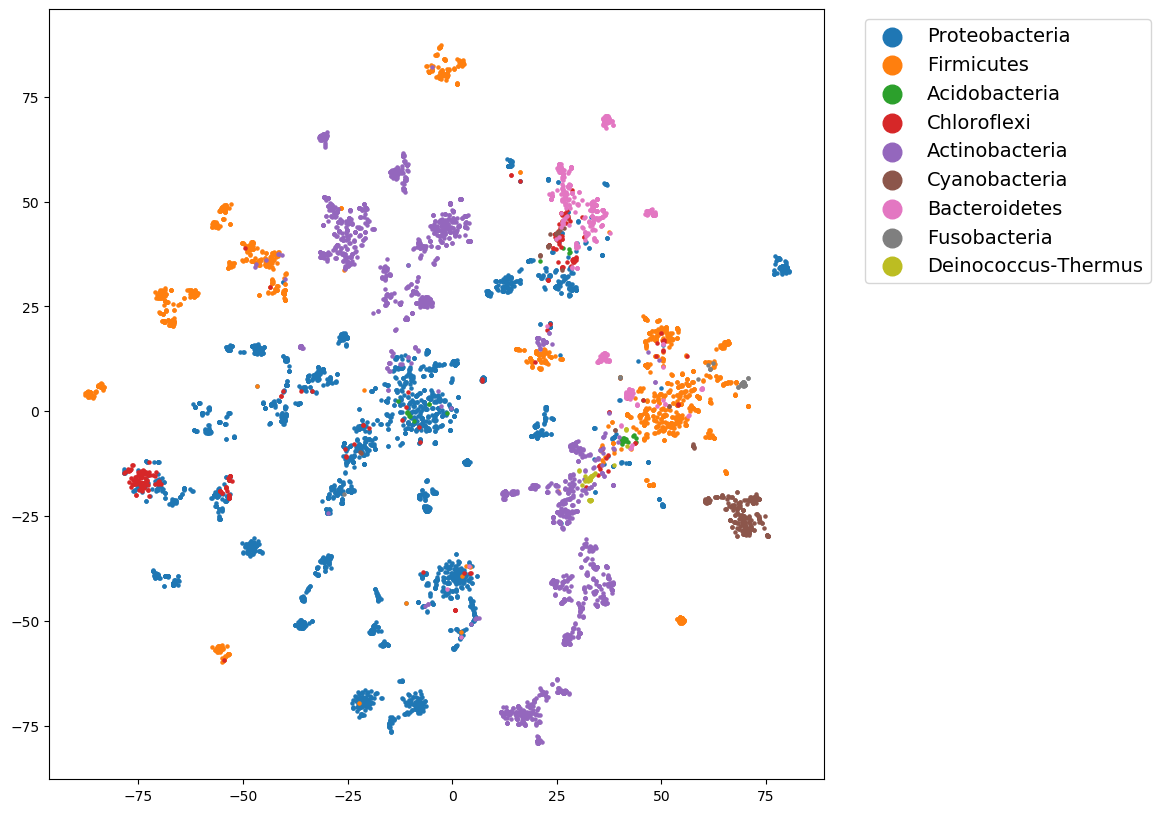
\includegraphics[width = \linewidth]{report/figures/unirep_tsne.png}
    \caption{A t-SNE visualization of UniRep's representation on selected phylums of $\beta$-lactamase.}
    \label{fig:unirep_tsne}
\end{figure}

Finally, in order to assess the significance of weighted sampling, we applied a weighted UniRep ensemble over $\beta$-lactamase, using alignment weights during training. The resulting correlation with experiments jumped to 0.594 under these settings.

\subsubsection{TAPE}
We train using TAPE's own training framework and TAPE's own validation sets. We then evaluate on TAPE's testing sets. The resulting scores can be seen in table \ref{tab:unirep_tape_results}.

\begin{table}[ht]
    \centering
    \begin{tabularx}{\textwidth}{lrrrr}
    \hline
    \textbf{Configuration} & \textbf{Secondary Structure} & \textbf{Remote Homology} & \textbf{Fluorescence} & \textbf{Stability} \\ \hline
    Finetuned              & 0.67                         & 0.07                     & 0.34                  & 0.70 \\
    Pretrained             & \textbf{0.69}                & \textbf{0.18}            & 0.45                  & 0.66 \\
    Pre. + Fine.           & 0.68                         & 0.12                     & \textbf{0.67}         & \textbf{0.74} \\
    \hline
    \end{tabularx}
    \caption{UniRep's performance on the TAPE tasks.}
    \label{tab:unirep_tape_results}
\end{table}

\subsection{Discussion}
\subsubsection{Mutation Effect Prediction}
The effect of pretraining UniRep seems to depend heavily on the specific protein family. Pretraining alone is insufficient to achieve good performance on all the datasets. Pretraining alone fails miraculously on the BLAT ECOLX (0.02) and HSP82 (0.04) datasets -- we are unsure why pretraining is especially insufficient for these datasets. We hypothesize that the UniRef50 dataset used for pretraining somehow does not cover these families well or maybe it is covered but the rest of the data is counterproductive to learning on these families.

However, we are not surprised by the fact that pretraining alone does not lead to good performance on this task. Pretraining on the global scale may lead to the model learning only coarse features, which do not translate well onto the local protein family scale. This is supported by how dramatically the performance increases when finetuning on the individual families.

Using both pretraining and finetuning on the mutation effect prediction task seems to have inconsistent performance in comparison to just finetuning. Even when pretraining and finetuning leads to an increased performance, the difference is insignificant. In contrast, pretraining and finetuning seems to have a significantly bad effect on performance on the GAL4 family, in comparison to just finetuning (from 0.46 to 0.37). This is remedied by the ensemble however. The ensembles perform better than any of the 5 models alone. This is consistent with our expectation that ensemble models perform better in general.

Overall, the finetuned UniRep achieves a performance on the mutation effect prediction task comparable to the reference correlation (table \ref{tab:datasets}) on 3 out of 5 datasets, while falling short on BLAT ECOLX and RASH HUMAN. It performs better than the reference on the CALM1 HUMAN and GAL4 datasets, which we find surprising since we did not expect UniRep to be able to capture the local landscape very well. Still, UniRep seems unable to achieve truly high (>0.6) correlation coefficients.

The t-SNE visualization of the UniRep representations in figure \ref{fig:unirep_tsne} shows a clear separation of the phylums into clusters, with only few overlaps. We found this result somewhat surprising, as we did not believe the UniRep representation to be so nuanced, considering that the mean over the hidden states of the LSTM is a somewhat destructive operation. Using a linear dimensionality reduction (like principal components analysis) does not result in neatly clustered points. The t-SNE is a non-linear dimensionality reduction, and so the non-linear part of the transformation seems significant. This suggests that while the representations indeed carry the potential to distinguish classes of proteins, extra (non-linear) capacity is needed to achieve this. If these representations were to be used in practical settings, it might be advisable to use sufficiently powerful models on top, as one would otherwise risk that the representations are not ``fully understood'' by the model. This also raises the question of whether such non-linear transformations could be integrated into the representations themselves, instead of being an external requirement of the model using the representation. This is in correspondence with the primitive construction of the UniRep representation -- it is, after all, simply a mean over the LSTM's hidden states. This construction is a destructive operation and does not inherently have any properties that would make it easily linearly separable.

\subsubsection{TAPE}
On the TAPE tasks, pretraining seems beneficial, leading to significant performance boosts in the remote homology task (from 0.07 to 0.12) and the fluorescence task (from 0.34 to 0.67). For the remote homology task especially, this fits with expectations, as a global perspective may help in dividing proteins among folds, which are essentially a larger scale protein family. The pretrained and finetuned model achieves a performance on the stability task (0.74) which is slightly higher than the state-of-the-art models on TAPE's leaderboard\footnote{See \url{https://github.com/songlab-cal/tape}} (0.73). However, the performance on the other tasks are not as impressive.

Surprisingly, finetuning after pretraining seems to lead to significantly worse performance on the remote homology task (from 0.18 to 0.12) -- it may be that the model is more prone to overfitting when given the opportunity to train the top model as well as the inner UniRep model. Across tasks, global pretraining provided by the UniRef50 dataset seems beneficial for tasks like TAPE, which is not too surprising as the tasks use data across protein families. UniRep's performance can be significantly better on the TAPE tasks using a smarter representation, as evidenced by TAPE's own UniRep implementation which uses an attention-weighted mean as its representation. This suggests that the mean representation we use is not ideal. The other change that could play a role is the down-scaling of the representation size. We do not know how these two interrelate with respect to the observed performance. This could be investigated by simply either changing how the representation is performed, or changing the size of the representation.

\section{Variational Autoencoder}
\label{sec:variational_autoencoders_experiement}
We trained the VAE on the five protein families, varying whether the models apply MAP weight estimates or full Bayesian weight estimates. In addition we also test with- and without sparse interaction. Finally, we noticed that it is significant whether samples are batch sampled according to their weights and evenly weighted in their contribution to the loss function, or whether samples are batched uniformly at random without replacement, and then scaled in the loss function according to their weights. This difference is explicit in our results as well. We briefly explain the difference here, for a protein family $\ve{P} = p_1, \ldots, p_n$ of $n$ samples, with weights $\ve{\pi} = \pi_1, \ldots, \pi_n$, where $\sum_{i = 1}^n \pi_i = 1$. With random weighted sampling (rws), the batch and loss calculation is as follows:
\begin{enumerate}
    \item Sample a set $\ve{T}$ of $n$ training candidates from $\ve{P}$ according to $\ve{\pi}$, with replacement.
    \item Train the model $f$ on $\ve{T}$ using mini-batches. For a batch $\ve{B} = b_1, \ldots, b_m$, the loss is the mean of the individual batch sample losses, i.e. for a loss function $\mathcal{L}$ we have a batch loss of 
    \[ \frac{1}{m}\sum_{i = 1}^{m} \mathcal{L}(f(b_i), b_i).\]
\end{enumerate}
Without random weighted sampling, the batch and loss calculation is slightly different:
\begin{enumerate}
    \item Let $\ve{T} = \ve{P}$.
    \item Train the model $f$ on $\ve{T}$ using mini-batches. For a batch $\ve{B} = b_1, \ldots, b_m$, the loss is the weighted mean of the individual batch sample losses according to their weights in $\ve{\pi}$, i.e. for a loss function $\mathcal{L}$ we have a batch loss of 
    \[ \sum_{i = 1}^{m} \pi_{b_i} \mathcal{L}(f(b_i), b_i).\]
\end{enumerate}
It may seem that these two procedures are equivalent, but in practical settings the two yield different performance results, likely because of the variation on weight updates.

The training process uses both the encoder and the decoder. The encoder compresses the sequence from its original size (that is, a flattened one-hot encoding) into two 1500-dimensional layers, before reaching the 30-dimensional latent representation distribution, represented by two 30-dimensional linear layers, respectively denoting the mean and log-variance of the latent representation. Samples are drawn from the representation, which are sent into the decoder. The decoder has a 100-dimensional layer, followed by a 2000-dimensional layer, before reaching the original sequence size again. The architecture is illustrated in figure \ref{fig:vae_architecture}.

\begin{figure}[H]
    \centering
    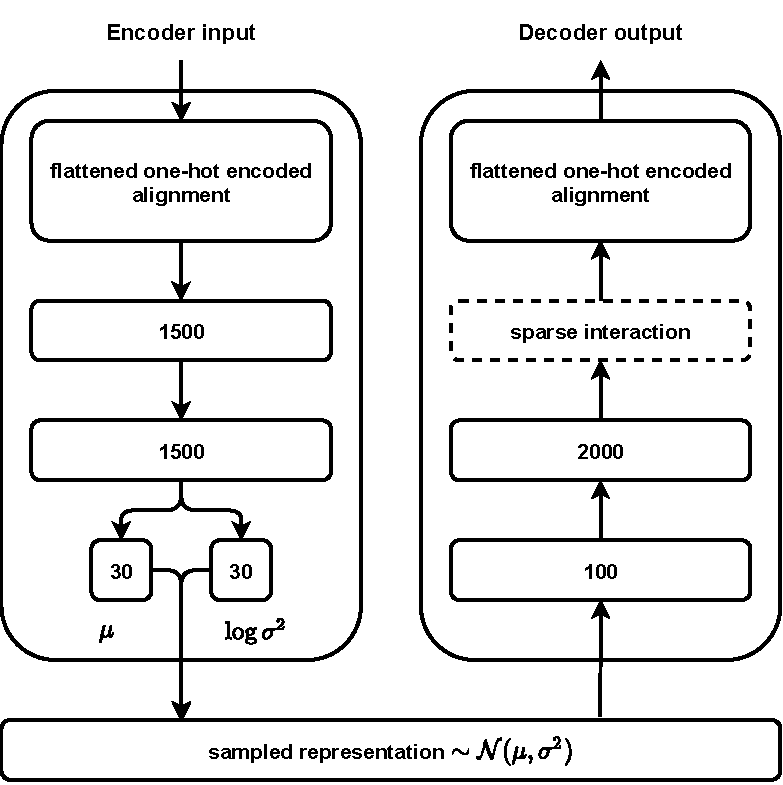
\includegraphics{report/figures/VAE_architecture2.pdf}
    \caption{Architecture of the VAE model.}
    \label{fig:vae_architecture}
\end{figure}

\subsection{Results}
As an initial sanity check, we wanted to inspect the representations produced by the VAE. To do this, we constructed a VAE model with a 2-dimensional latent space and plotted the resulting representations. Even in two dimensions, a plot of desirable protein representations should show similar proteins clustered together (and hence dissimilar proteins well at distance). Figure \ref{fig:2dimvae} shows the mean of the representations of proteins from the $\beta$-lactamase protein family, colored by phylum, as produced by this model. The structure of the representations resemble that of a phylogenetic tree, suggesting that the model correctly identifies the evolutionary similarities between the different variants of $\beta$-lactamase. A similar phylogenetic tree-like structure is seen when using the model on other protein families. In addition, small mutations in a protein should yield representations that lie relatively close to the unmutated protein they come from. This is shown in the zoomed subregion of figure \ref{fig:2dimvae}, where the wild type (i.e. unmutated) protein is shown together with its mutations. 

\begin{figure}[H]
    \centering
    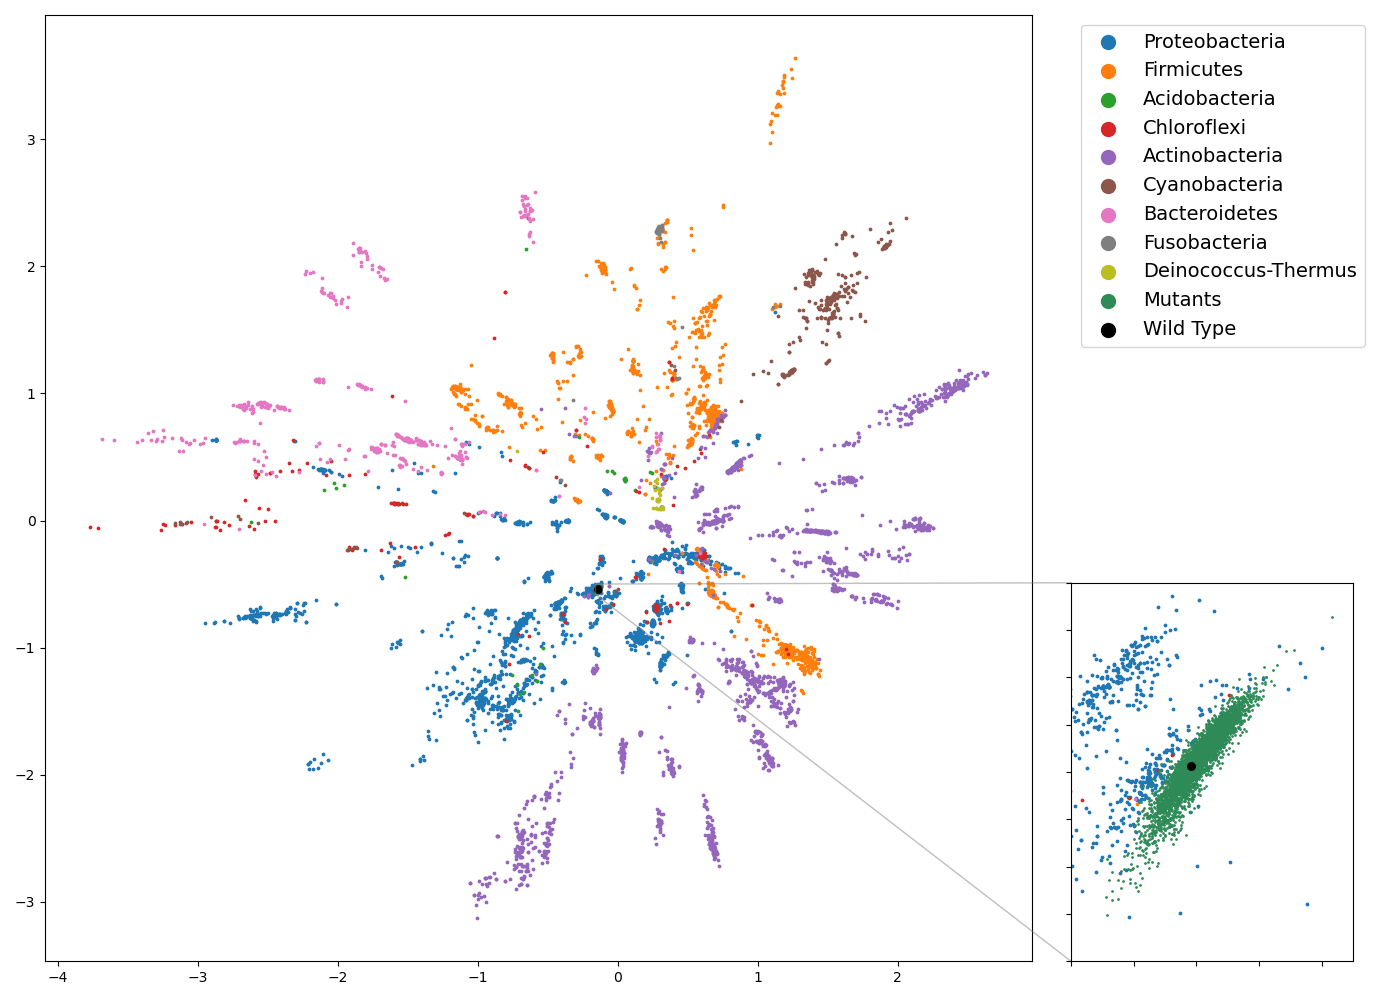
\includegraphics[width = \linewidth]{report/figures/family_and_mutations.png}
    \caption{Mean of the protein representations of selected phylums of $\beta$-lactamase, produced by a VAE model with a bottleneck layer size of 2. The subregion to the right is a zoom of the representations of the wild type mutants (shown in green).}
    \label{fig:2dimvae}
\end{figure}

In table \ref{tab:vae_results} we display the collected mutation effect prediction correlation results across models and protein families. Each result is the average over 5 models trained with the same settings to adjust for random initialization and other factors contributing to variance in the performance. The full results of single training and testing sessions can be found in appendix \ref{appendix}.
\begin{table}[H]
    \centering
    \begin{tabularx}{\textwidth}{lrrrrr}
    \hline
    \textbf{Configuration} & \textbf{BLAT ECOLX} & \textbf{CALM1 HUMAN} & \textbf{GAL4} & \textbf{HSP82} & \textbf{RASH HUMAN} \\ \hline
    \textbf{MAP} & 0.57 & 0.28 & 0.39 & 0.47 & 0.49 \\
    \textbf{MAP + sparse} & 0.66 & \textbf{0.29} & 0.47 & 0.49 & 0.47 \\
    \textbf{MAP + sparse + rws} & 0.69 & \textbf{0.29} & 0.48 & 0.51 & 0.40 \\
    \textbf{Bayes} & 0.69 & 0.27 & 0.37 & 0.47 & \textbf{0.50} \\
    \textbf{Bayes + sparse} & 0.71 & 0.27 & 0.37 & 0.51 & 0.38 \\
    \textbf{Bayes + sparse + rws} & 0.73 & 0.26 & 0.61 & \textbf{0.55} & 0.49 \\
    \textbf{Bayes ensemble} & 0.77 & 0.27 & \textbf{0.63} & \textbf{0.55} & 0.48 \\
    \hline
    \textbf{DeepSequence \cite{riesselman2018deep}} & \textbf{0.78} & 0.23 & 0.45 & 0.53 & 0.47 \\
    \hline
    \end{tabularx}
    \caption{Mutation effect prediction correlation using variants of the VAE model. Each measure is averaged over five sessions. DeepSequence prediction correlations are provided as a reference. \textit{Bayes ensemble} refers to the ensemble over the 5 sessions of Bayes + sparse + rws, rather than the average.}
    \label{tab:vae_results}
\end{table}

Overall, the full Bayesian weight treatment seem to improve the performance across the datasets. The results are discussed in detail in section \ref{sec:vae_results_discussion}.

The model is explicitly trained to reconstruct its input protein sequence from its encoded representation. In figure \ref{fig:protein_reconstruction} the $\beta$-lactamase query protein is shown along with its reconstruction.
\begin{figure}[H]
    \centering
    \texttt{1--80 \\
HPETLVKVKDAEDQLGARVGYIELDLNSGKILESFRPEERFPMMSTFKVLLCGAVLSRVDAGQEQLGRRIHYSQNDLVEY \\
\textcolor{red}{.}\textcolor{red}{.}\textcolor{red}{.}\textcolor{red}{L}\textcolor{red}{A}\textcolor{red}{E}\textcolor{red}{T}\textcolor{green}{V}\textcolor{green}{K}\textcolor{red}{Q}\textcolor{green}{A}\textcolor{green}{E}\textcolor{red}{K}\textcolor{red}{R}\textcolor{green}{L}\textcolor{green}{G}\textcolor{green}{A}\textcolor{green}{R}\textcolor{green}{V}\textcolor{green}{G}\textcolor{green}{Y}\textcolor{red}{A}\textcolor{green}{E}\textcolor{green}{L}\textcolor{green}{D}\textcolor{green}{L}\textcolor{red}{A}\textcolor{green}{S}\textcolor{green}{G}\textcolor{green}{K}\textcolor{red}{L}\textcolor{green}{L}\textcolor{green}{E}\textcolor{green}{S}\textcolor{red}{Y}\textcolor{green}{R}\textcolor{red}{A}\textcolor{red}{D}\textcolor{green}{E}\textcolor{green}{R}\textcolor{green}{F}\textcolor{green}{P}\textcolor{green}{M}\textcolor{green}{M}\textcolor{green}{S}\textcolor{green}{T}\textcolor{green}{F}\textcolor{green}{K}\textcolor{green}{V}\textcolor{green}{L}\textcolor{green}{L}\textcolor{green}{C}\textcolor{green}{G}\textcolor{green}{A}\textcolor{green}{V}\textcolor{green}{L}\textcolor{red}{A}\textcolor{green}{R}\textcolor{green}{V}\textcolor{green}{D}\textcolor{green}{A}\textcolor{green}{G}\textcolor{red}{E}\textcolor{green}{E}\textcolor{green}{Q}\textcolor{green}{L}\textcolor{red}{D}\textcolor{green}{R}\textcolor{green}{R}\textcolor{green}{I}\textcolor{red}{T}\textcolor{green}{Y}\textcolor{red}{R}\textcolor{red}{K}\textcolor{red}{S}\textcolor{green}{D}\textcolor{green}{L}\textcolor{green}{V}\textcolor{green}{E}\textcolor{green}{Y} \\
81--160 \\
SPVTEKHLTDGMTVRELCSAAITMSDNTAANLLLTTIGGPKELTAFLHNMGDHVTRLDRWEPELNEAIPNDERDTTMPAA \\
\textcolor{green}{S}\textcolor{green}{P}\textcolor{green}{V}\textcolor{green}{T}\textcolor{green}{E}\textcolor{green}{K}\textcolor{green}{H}\textcolor{green}{L}\textcolor{red}{A}\textcolor{green}{D}\textcolor{green}{G}\textcolor{green}{M}\textcolor{green}{T}\textcolor{green}{V}\textcolor{red}{A}\textcolor{green}{E}\textcolor{green}{L}\textcolor{green}{C}\textcolor{red}{E}\textcolor{green}{A}\textcolor{green}{A}\textcolor{green}{I}\textcolor{green}{T}\textcolor{green}{M}\textcolor{green}{S}\textcolor{green}{D}\textcolor{green}{N}\textcolor{green}{T}\textcolor{green}{A}\textcolor{green}{A}\textcolor{green}{N}\textcolor{green}{L}\textcolor{green}{L}\textcolor{green}{L}\textcolor{red}{A}\textcolor{red}{S}\textcolor{green}{I}\textcolor{green}{G}\textcolor{green}{G}\textcolor{green}{P}\textcolor{red}{A}\textcolor{red}{G}\textcolor{green}{L}\textcolor{green}{T}\textcolor{green}{A}\textcolor{green}{F}\textcolor{green}{L}\textcolor{red}{R}\textcolor{red}{S}\textcolor{red}{I}\textcolor{green}{G}\textcolor{green}{D}\textcolor{red}{T}\textcolor{green}{V}\textcolor{green}{T}\textcolor{green}{R}\textcolor{green}{L}\textcolor{green}{D}\textcolor{green}{R}\textcolor{green}{W}\textcolor{green}{E}\textcolor{green}{P}\textcolor{green}{E}\textcolor{green}{L}\textcolor{green}{N}\textcolor{green}{E}\textcolor{green}{A}\textcolor{red}{L}\textcolor{green}{P}\textcolor{red}{G}\textcolor{green}{D}\textcolor{green}{E}\textcolor{green}{R}\textcolor{green}{D}\textcolor{green}{T}\textcolor{green}{T}\textcolor{red}{T}\textcolor{green}{P}\textcolor{green}{A}\textcolor{green}{A} \\
161--240 \\
MATTLRKLLTGELLTLASRQQLIDWMEADKVAGPLLRSALPAGWFIADKSGAGERGSRGIIAALGPDGKPSRIVVIYTTG \\
\textcolor{green}{M}\textcolor{green}{A}\textcolor{red}{A}\textcolor{green}{T}\textcolor{green}{L}\textcolor{green}{R}\textcolor{green}{K}\textcolor{green}{L}\textcolor{green}{L}\textcolor{green}{T}\textcolor{green}{G}\textcolor{red}{D}\textcolor{red}{V}\textcolor{green}{L}\textcolor{red}{S}\textcolor{red}{P}\textcolor{green}{A}\textcolor{green}{S}\textcolor{green}{R}\textcolor{green}{Q}\textcolor{green}{Q}\textcolor{green}{L}\textcolor{green}{I}\textcolor{green}{D}\textcolor{green}{W}\textcolor{green}{M}\textcolor{red}{V}\textcolor{green}{A}\textcolor{green}{D}\textcolor{green}{K}\textcolor{green}{V}\textcolor{green}{A}\textcolor{green}{G}\textcolor{green}{P}\textcolor{green}{L}\textcolor{green}{L}\textcolor{green}{R}\textcolor{green}{S}\textcolor{red}{V}\textcolor{green}{L}\textcolor{green}{P}\textcolor{green}{A}\textcolor{green}{G}\textcolor{green}{W}\textcolor{green}{F}\textcolor{green}{I}\textcolor{green}{A}\textcolor{green}{D}\textcolor{green}{K}\textcolor{red}{T}\textcolor{green}{G}\textcolor{green}{A}\textcolor{green}{G}\textcolor{green}{E}\textcolor{green}{R}\textcolor{green}{G}\textcolor{green}{S}\textcolor{green}{R}\textcolor{green}{G}\textcolor{green}{I}\textcolor{green}{I}\textcolor{green}{A}\textcolor{red}{V}\textcolor{green}{L}\textcolor{green}{G}\textcolor{green}{P}\textcolor{green}{D}\textcolor{green}{G}\textcolor{green}{K}\textcolor{green}{P}\textcolor{green}{S}\textcolor{green}{R}\textcolor{green}{I}\textcolor{green}{V}\textcolor{green}{V}\textcolor{green}{I}\textcolor{green}{Y}\textcolor{red}{L}\textcolor{green}{T}\textcolor{red}{E} \\
241--263 \\
SQATMDERNRQIAEIGASLIKHW \\
\textcolor{red}{T}\textcolor{red}{E}\textcolor{green}{A}\textcolor{green}{T}\textcolor{green}{M}\textcolor{green}{D}\textcolor{green}{E}\textcolor{green}{R}\textcolor{green}{N}\textcolor{red}{A}\textcolor{green}{Q}\textcolor{green}{I}\textcolor{green}{A}\textcolor{green}{E}\textcolor{green}{I}\textcolor{green}{G}\textcolor{green}{A}\textcolor{red}{A}\textcolor{green}{L}\textcolor{green}{I}\textcolor{green}{K}\textcolor{green}{H}\textcolor{green}{W}}
    \caption{Reconstruction of the $\beta$-lactamase query protein by the ensembled VAE model. The reconstruction is by the ensemble of models with decoder weights sampled from the learned weight distributions. The top sequence is the original, while the bottom is the reconstructed sequence. Red and green positions denote incorrect and correct reconstruction, respectively. The accuracy is $\approx 80\%$.}
    \label{fig:protein_reconstruction}
\end{figure}


In a similar fashion, we found it important to inspect the likelihood predictions produced by the model. The positional predictions of a random subsample of 4 protein sequences from $\beta$-lactamase is shown in figure \ref{fig:softmax}.
\begin{figure}[H]
    \centering
    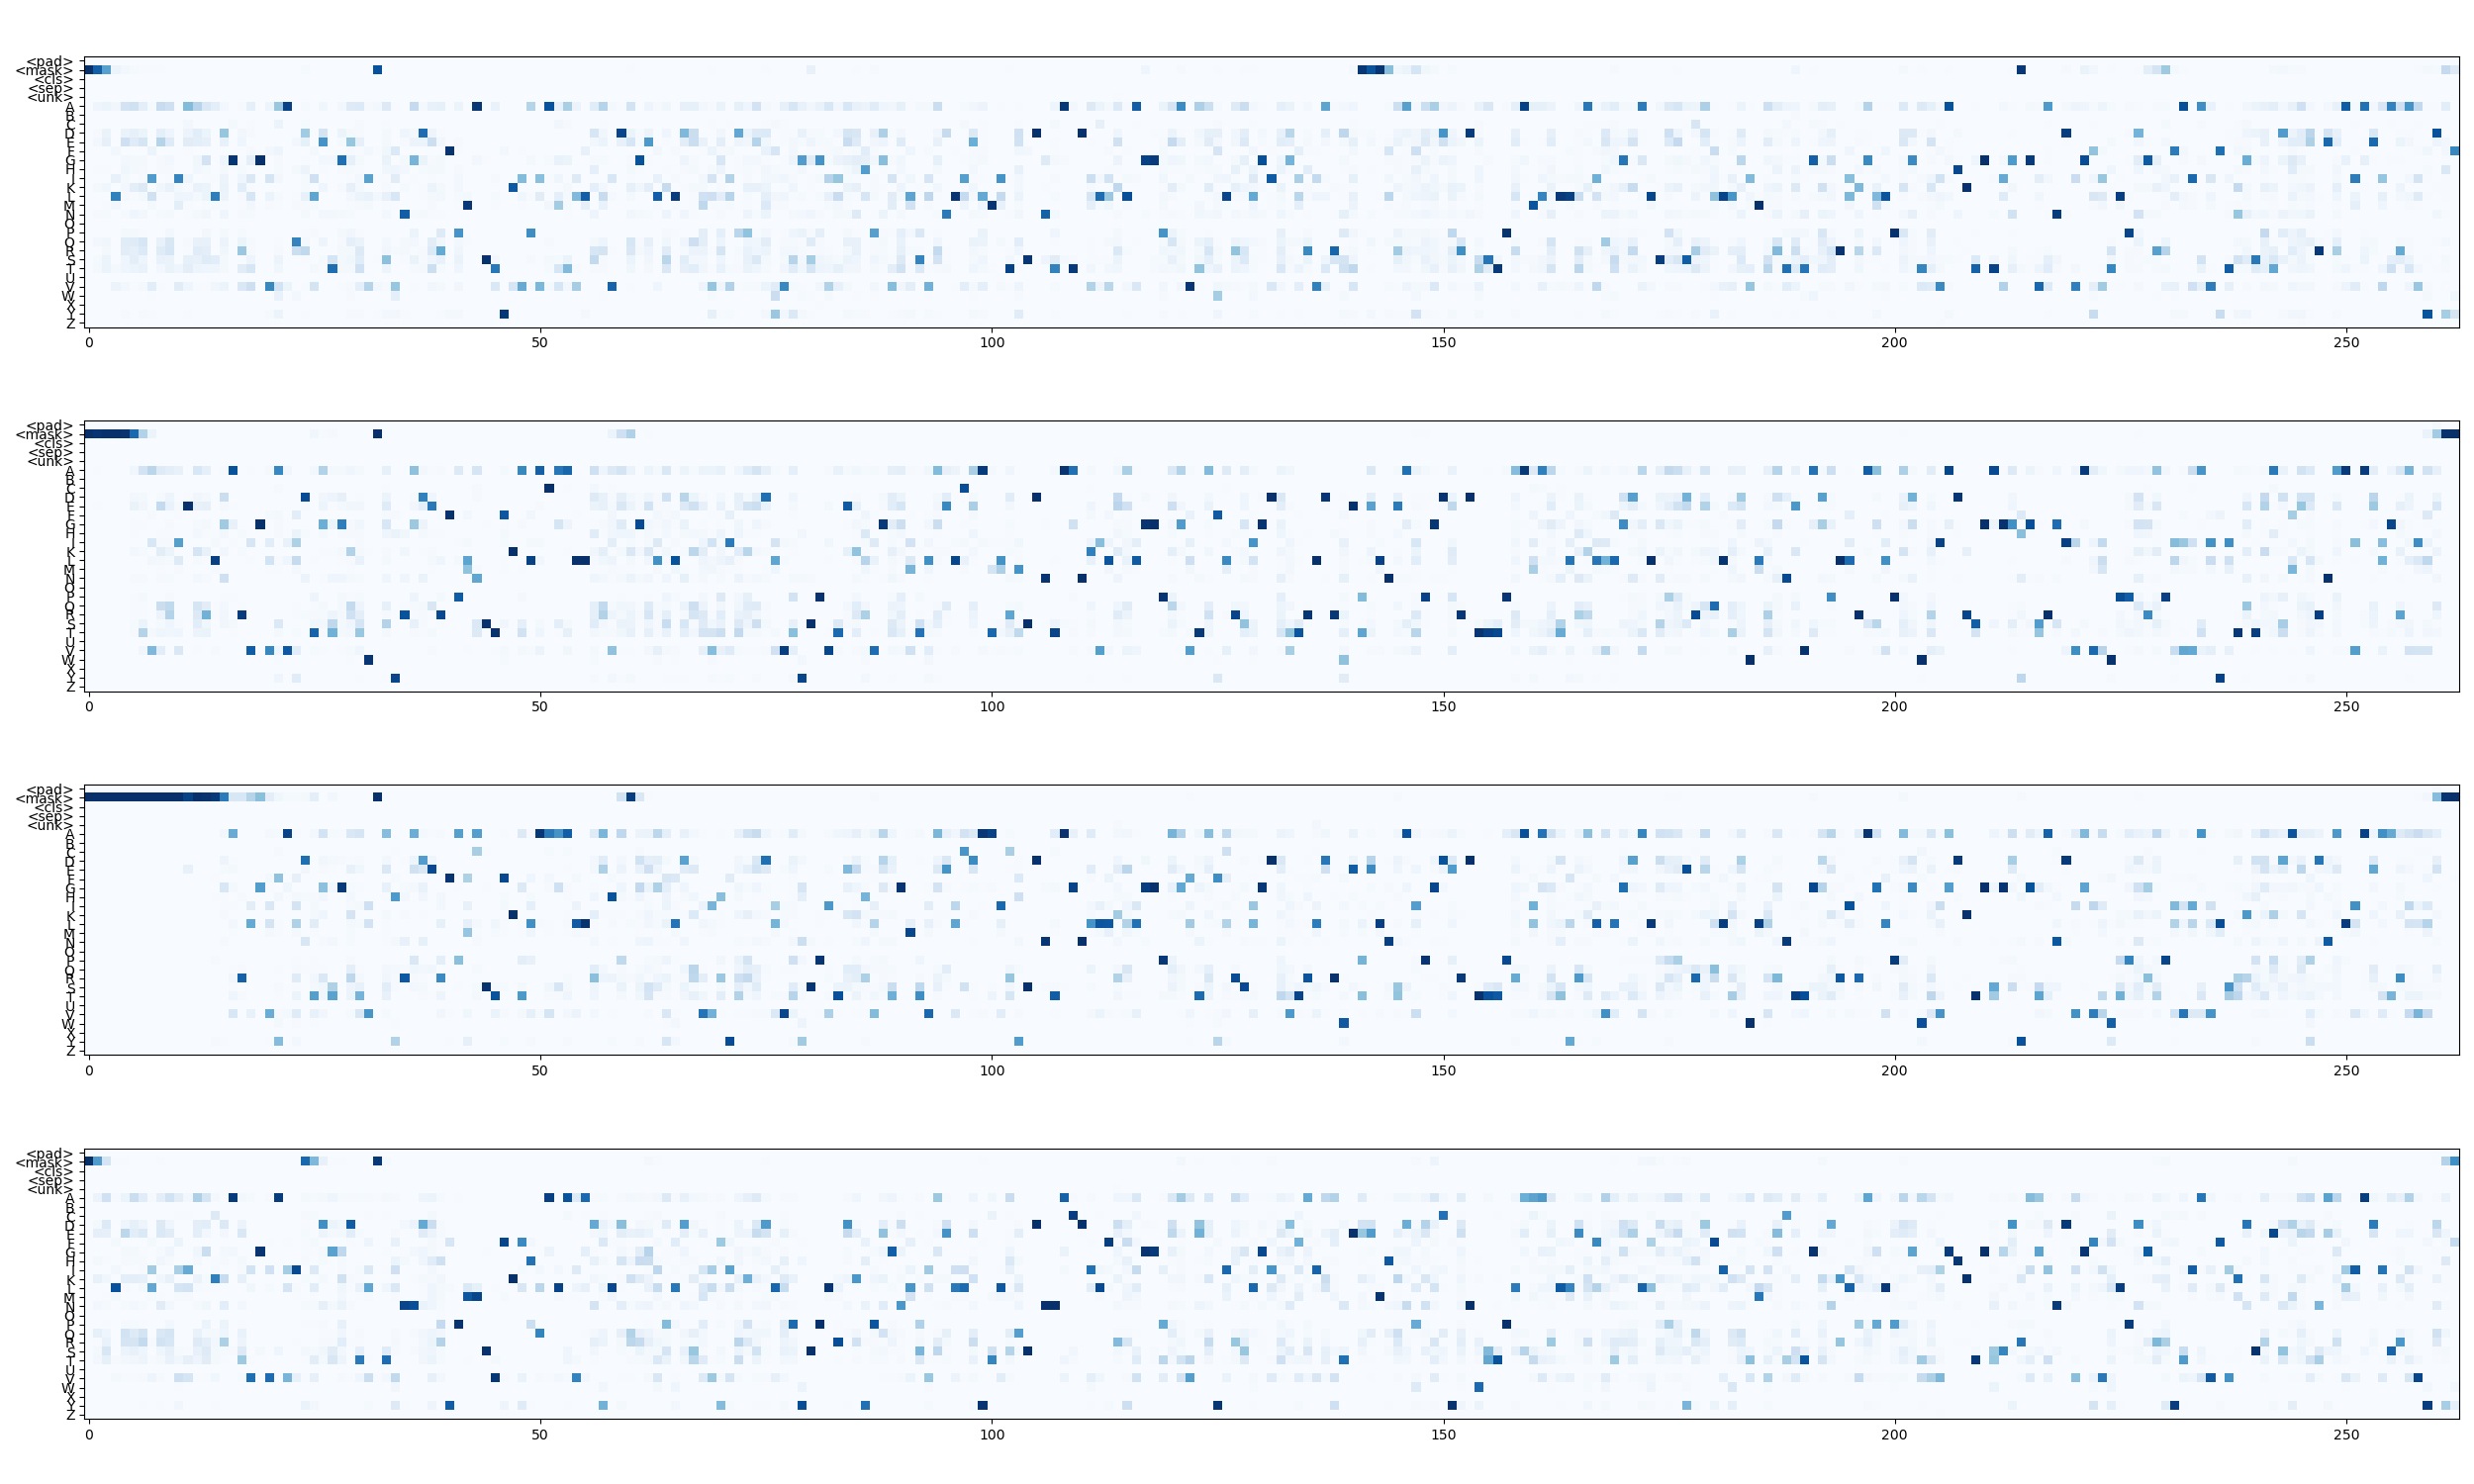
\includegraphics[width = 0.9\linewidth]{report/figures/softmax.png}
    \caption{Softmax predictions on 4 protein sequences from the $\beta$-lactamase protein family. The figure does not afford close inspection, but it suffices as a sanity check that the model does indeed produce complex distributions over the potential amino acids at each position. The intensity of blue denotes more likely predictions.}
    \label{fig:softmax}
\end{figure}

\subsection{Discussion}
\label{sec:vae_results_discussion}

This section contains discussion mainly focused on the experiments related to the VAE and its produced representation. The general discussion across experiments can be found in chapter \ref{chapter:experiments}.

Because the VAE is constrained to aligned, fixed-length protein sequences, they do not generalize to the tasks in the TAPE benchmark, which unfortunately means that we will currently not be able to assess how well this approach perform on these tasks. This is entirely because the current setup does not allow inputs of variable lengths. In section \ref{sec:extracting_representations} we sketch potential future work that might resolve these limitations.

\subsubsection{Mutation Effect Predictions}
This part of the discussion refers to figure \ref{tab:vae_results}. In our experiments, yielding a correlation coefficient above 0.70 on the $\beta$-lactamase protein family required Bayesian weight estimates, while MAP estimates with sparse interaction and random weighted samples is close at 0.69. The fact that Bayesian networks perform better than networks that produce MAP estimates, is in accordance with our expectations: the Bayesian model is an ensemble over networks, and so gain the benefit of ensembles. Specifically, it should reduce bias in the predictions, as these tend to be averaged out across the ensemble networks. It should also reduce variance in predictions as the number of models in the ensemble increases. That is, if you have a single protein sequence and ask many individual models for predictions, the variance of these predictions will be larger than the variance in predictions of many ensemble models. Sparse interactions seem to make a difference for MAP estimates on $\beta$-lactamase and GAL4, but there is no clear-cut conclusion to the merits of this feature. E.g. for RASH HUMAN, Bayesian predictions decline from 0.50 to 0.38 when sparse interactions are applied.

Across protein families, the correlation coefficient varies significantly, from 0.77 to 0.26. We have not been able to identify explanatory factors for this; it is likely that such explanations can be found in the relationship between the experimental metrics and the prediction metric. That is, equation \ref{eq:prediction_metric} might simply correlate better with the specific $\beta$-lactamase experimental measures and less so with CALM1 experimental data. On the surface, there is no clear relationship between results and the sizes of the families, nor their mutations.

In general our produced results are in accordance with what is achieved by \textcite{riesselman2018deep}. For all protein families but $\beta$-lactamase, we observe a relative increase in performance. The increase does however not seem to be significant, and might simply be due to variance. One noteable difference is on GAL4, where \textcite{riesselman2018deep} achieve 0.45 and our Bayesian VAE yields 0.61. The results should be directly comparable and so this difference is a little surprising. Note that every other VAE variant than random weighted sampling, sparse, Bayesian VAE are much closer to the reference predictions by \textcite{riesselman2018deep}. These are however minor observations to the general trend that the VAE model architecture seem to capture protein characteristics that correlate with experimental observations.

\subsubsection{Explained Variance of representation principal components}
A notable observation is that if principal component analysis is applied to the representations of the protein family, one can observe that the variance of the representations can be fully explained by 12 components, as seen in figure \ref{fig:explained_variance}. This raises some questions about the size of the latent space, and whether one could get similar performance with a smaller dimensionality. Additionally, this might also indicate that the model is not fully utilizing the capacity of the representation or that the signal from the data is not strong enough, as it seems implausible that we can accurately and compactly represent proteins in 12 dimensions. It may also be that the model does utilize the remaining 18 dimensions, but that the values the model uses in those dimensions are much smaller.
\begin{figure}[H]
    \centering
    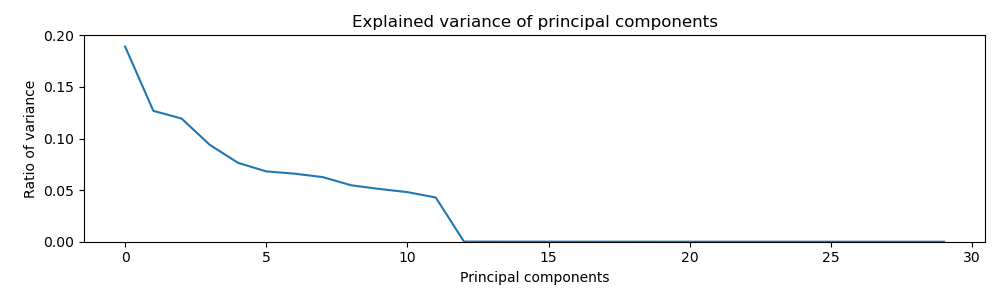
\includegraphics[width = \linewidth]{report/figures/explained_variance.png}
    \caption{Explained variance of the principal components of the 30-dimensional representations of the BLAT ECOLX protein family.}
    \label{fig:explained_variance}
\end{figure}

\subsubsection{Bayesian Weight Distributions}
Because the Bayesian VAE seem to improve performance, we thought it made sense to inspect the learned distributions to see if there was anything worth noting. In figure \ref{fig:bayesian_weights}, learned weight distributions of two decoder neurons are shown. Some neurons have weights diversely distributed, indicating that the neuron has learned useful weight distributions in relation to the task of reconstructing its input sequences. However, other neurons seem to carry weights that are all closely distributed as a unit Gaussian. Such neurons are the most common. This is not really surprising, as the model is explicitly trained to minimize the divergence between its weight distributions and the weight prior, a unit Gaussian. However, this behavior suggests that a significant part of the model capacity is used to fulfill the pull of the prior distribution. The prior was chosen solely for convenience, and this choice seems to affect the weight distributions more than desired. It is unlikely that the model effectively utilizes weights that are in expectation zero, and thus almost equally likely to be positive or negative. For these reasons, the architecture might benefit from choosing other weight priors. An initial choice could be the scale mixture as suggested by \textcite{blundell2015weight}.

This is also an indication that the network could be compressed by a procedure that eliminates weights that are distributed sufficiently close to a unit Gaussian distribution, as these weights are unlikely to contribute to the prediction behavior of the network. This might be related to some of the ideas proposed in \textcite{molchanov2017variational, kingma2015variational, gal2016dropout}, where model compression, dropout and the Bayesian approach are shown to be connected -- this is outside our scope however, so we leave this as an interesting observation and potentially the foundation for future work.

% In \cite{gal2016dropout}, dropout and Bayesian neural networks are shown to be connected, while it is shown in \cite{kingma2015variational} that Gaussian dropout can be learned and that this often makes networks more effective during training. Finally, it is shown in \cite{molchanov2017variational} that such dropout can be used to make networks more sparse, giving merit to the idea of using Bayesian weights to compress a network. \{approve this insanity}

\begin{figure}[H]
    \centering
    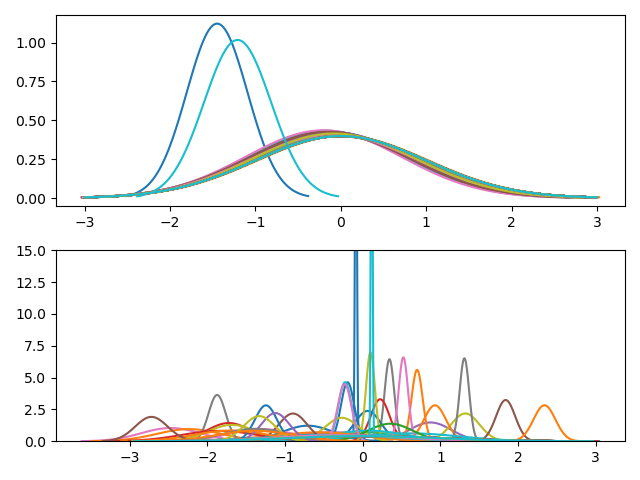
\includegraphics[width = 0.8\linewidth]{report/figures/bayesian_weighs.png}
    \caption{\textit{Top:} Weight distributions of the first neuron of the 2000-sized linear layer of the decoder. Almost all its weights are closely shaped to a unit Gaussian distribution, likely an effect of the prior being unit Gaussian and a training objective that minimizes the KL divergence to the prior. \textit{Bottom:} The 32nd neuron in the same layer. Here weight distributions are much more diverse, suggesting that this neuron is critical. Neurons similar to the first neuron are most commonly observed in the layer. Each neuron has 100 weights.}
    \label{fig:bayesian_weights}
\end{figure}

\section{WaveNet}
\label{sec:wavenet_experiment}
Like UniRep and the VAE, the WaveNet model architecture was trained on each of the five chosen protein family datasets (see section \ref{sec:data}) for mutation effect prediction. The mutation effect experiments are conducted by training the model to reconstruct sequence inputs, compelling the model to learn factors that drive protein characteristics. For a given input sequence, the model predicts each residue position based on the sequence observed so far at that position. We trained a total of 6 models: 3 observing sequences in a ``forward'' direction (N-terminus to C-terminus), and 3 observing sequences in a ``backward'' direction (C-terminus to N-terminus). This ensemble of models determine the mutation effect predictions. We have adopted hyperparameter settings as described in \textcite{riesselman2019accelerating}, using L2 regularization of model parameters with coefficient $\lambda = 1$, a clipping of gradient norms to 100, and an aggressive dropout probability of $\sfrac{1}{2}$ on model components. The WaveNet architecture was instantiated with a dilation stack of 6 dilation blocks, each consisting of 9 dilation layers (that is, dilation in the range $1, 2, 4, \ldots, 256$). The number of channels used in the NormConv layers is 48 (with the exception of final and initial convolutions which map to and from the number of candidate residues).

In the case study of the $\beta$-lactamase protein family, we have two variants of the experiment: one where each protein sequence input is equally weighted in the loss calculation, and one with sequence weights according to sequence similarity (see \ref{sec:data} for details). This is in order to determine the significance of weighted samples on model performance. The weights are currently indirectly dependent on an alignment, and so cannot be assumed to be freely available in a general setting.

In addition another model instance was pretrained and/or finetuned for TAPE, in the same manner as the UniRep model. In this setting, the model architecture provides the representation for a top model. Collectively, this setup is trained on labeled TAPE training datasets and evaluated provided test sets, for each task.

For pretraining, we applied the model to the full UniRef50 dataset, without any regularization, for at least a full epoch. We did not use any regularization in the pretraining since the UniRef50 dataset is so huge that we believe that overfitting will not be a big problem. We did however use 1\% as validation, just like with UniRep.

\subsection{Results}

\subsubsection{Mutation Effect Prediction}
For this task, we train 6 models independently, 3 forwards and 3 backwards. We report both the mean of the models' results but we also combine them into an ensemble model to achieve stronger results. We used $20\%$ of the data samples as a validation set. The results can be seen in table \ref{tab:wavenet_rho_results}.

% The stopping criteria resulted in relatively short training sessions of less than 20 epochs. In the unweighted case, it is significant for performance to keep a low patience. This behavior is discussed further in \ref{sec:wavenet_discussion}. %The correlation coefficient $\rho$ between predictions and measured experiments steadily increase during training as seen in figure~\ref{fig:wn_f2_rho}~and~\ref{fig:wn_b2_rho}.

% \{should this even be here?}

% \begin{minipage}{\linewidth}
% 	\centering
% 	\begin{minipage}{0.49\linewidth}
% 		\begin{figure}[H]
% 			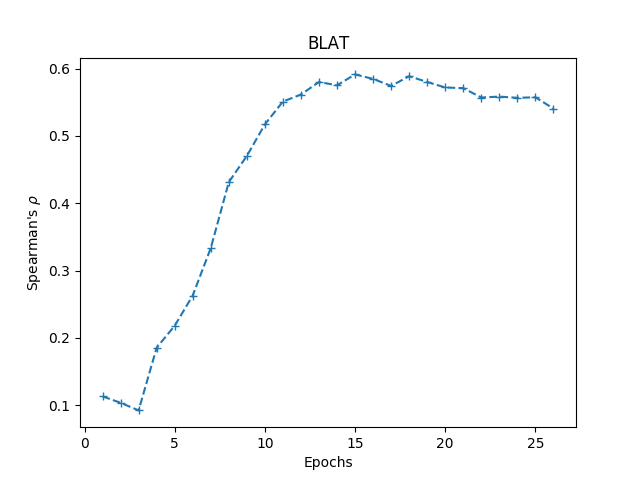
\includegraphics[width=\linewidth]{report/figures/wn_f2_rho.png}
% 			\caption{Forward-pass training correlation.}
% 		    \label{fig:wn_f2_rho}
% 		\end{figure}
% 	\end{minipage}
% 	\hfill
% 	\begin{minipage}{0.49\linewidth}
% 		\begin{figure}[H]
% 			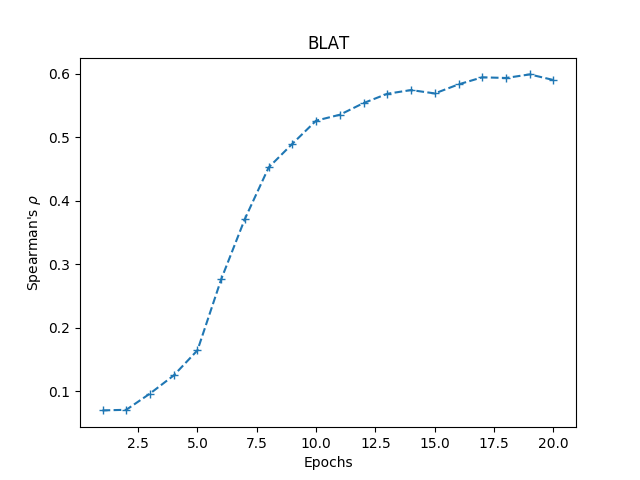
\includegraphics[width=\linewidth]{report/figures/wn_b2_rho.png}
% 		    \caption{Backward-pass training correlation.}
% 		    \label{fig:wn_b2_rho}
% 		\end{figure}
% 	\end{minipage}
% \end{minipage}

% For the unweighted models, the model mutation effect predictions have a Spearman $\rho$ correlation with experimental results of 0.627. For the weighted models, the mutation effect predictions have a correlation of 0.717. This indicates that sample weights provide a significant performance addition. This is discussed further in section \ref{sec:wavenet_discussion}.

\begin{table}[ht]
    \centering
    \begin{tabularx}{\textwidth}{lccccc}
    \hline
    \textbf{Configuration} & \textbf{BLAT ECOLX} & \textbf{CALM1 HUMAN} & \textbf{GAL4} & \textbf{HSP82} & \textbf{RASH HUMAN} \\ \hline
    Finetuned              & 0.56                & 0.27                 & 0.50          & 0.45           & 0.39 \\
    Pretrained             & 0.08                & 0.16                 & 0.04          & 0.06           & 0.33 \\
    Pre. + Fine.           & 0.50                & 0.27                 & 0.46          & 0.45           & 0.35 \\
    \hline
    Finetuned (E)          & \textbf{0.61}       & \textbf{0.29}        & \textbf{0.54} & \textbf{0.51}  & \textbf{0.43} \\
    Pre. + Fine. (E)       & 0.55                & \textbf{0.29}        & 0.49          & 0.50           & 0.40 \\
    \hline
    \end{tabularx}
    \caption{Mutation effect prediction Spearman's $\rho$ correlation scores for the WaveNet model on different datasets, on the different configurations. The bottom two rows indicate ensembles over the 6 models rather than averages.}
    \label{tab:wavenet_rho_results}
\end{table}
The pretrained only WaveNet variant achieve near to no correlation on most datasets, the exception being RASH HUMAN, where it performs comparably to the finetuned model. The best performing model is the finetuned ensemble, achieving 0.61 on BLAT, 0.29 on CALM1, 0.54 on GAL, 0.51 on HSP82 and 0.43 on RASH. Across the models, these are the highest correlations.

We also tried training a model on weighted samples of the $\beta$-lactamase family. If samples are weighted, the model performance increases significantly, from 0.61 to 0.72, suggesting that this is an important factor.

Just as with the other models, we have visualized WaveNet's representations of the $\beta$-lactamase family. This is a high-dimensional representation, in this case 48 dimensions, which requires us to use a dimensionality reduction. We use t-SNE, just as we did with UniRep. The result can be seen in figure~\ref{fig:wavenet_tsne}.

\begin{figure}[H]
    \centering
    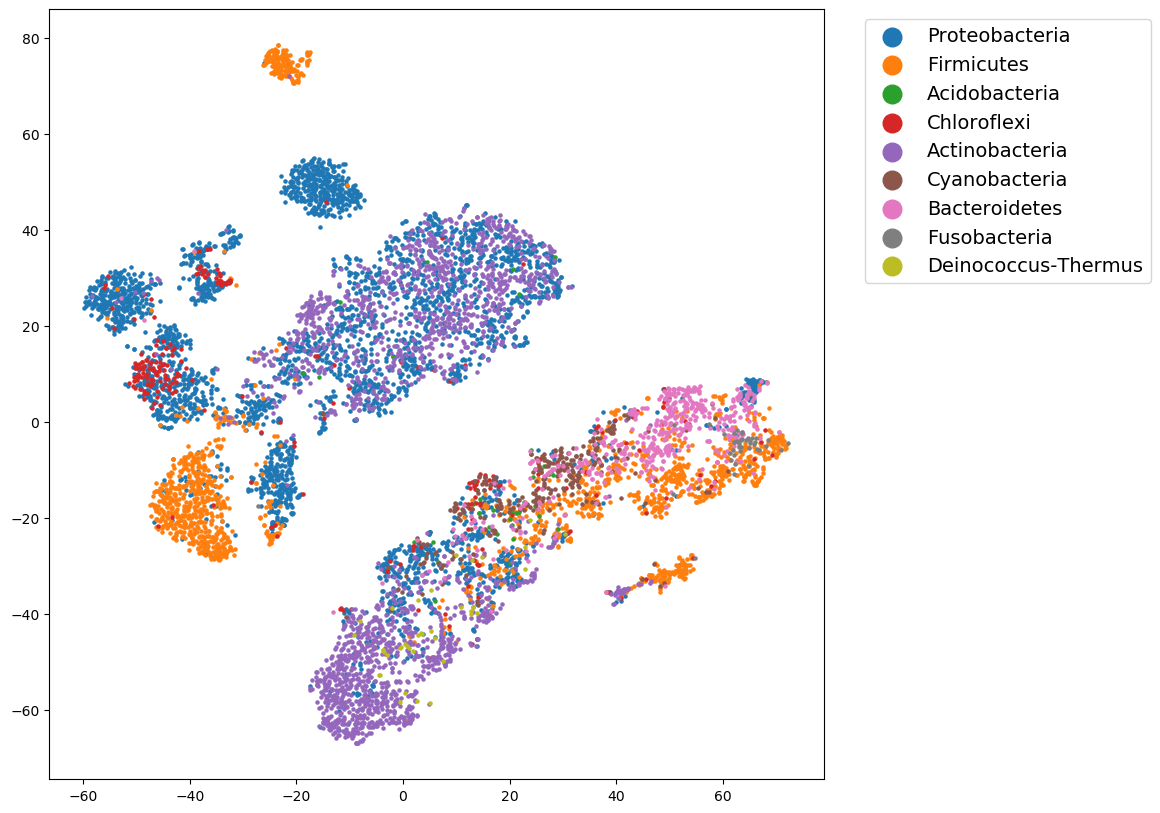
\includegraphics[width = \linewidth]{report/figures/wavenet_tsne.png}
    \caption{t-SNE visualization of one of the forwards WaveNet model's representations of the $\beta$-lactamase family.}
    \label{fig:wavenet_tsne}
\end{figure}

\subsubsection{TAPE}
When training WaveNet on TAPE, we only use a single forward model. Otherwise, we trained WaveNet on the TAPE tasks in the same way the UniRep model was trained. The results can be seen in figure~\ref{tab:wavenet_tape_results}.

\begin{table}[H]
    \centering
    \begin{tabularx}{0.93\textwidth}{lrrrr}
    \hline
    \textbf{Configuration} & \textbf{Secondary Structure} & \textbf{Remote Homology} & \textbf{Fluorescence} & \textbf{Stability} \\ \hline
    Finetune               & 0.35                         & 0.09                     & 0.07                  & \textbf{0.78} \\
    Pretrain               & \textbf{0.38}                & \textbf{0.17}            & \textbf{0.47}         & 0.58 \\
    Pre. + Fine.           & 0.35                         & 0.04                     & 0.32                  & 0.66 \\
    \hline
    \end{tabularx}
    \caption{WaveNet's performance on the TAPE tasks.}
    \label{tab:wavenet_tape_results}
\end{table}

\subsection{Discussion}
\label{sec:wavenet_discussion}

\subsubsection{Mutation Effect Prediction}
When sample-weights are applied, the WaveNet model performs comparatively to the VAE and DeepSequence on the $\beta$-lactamase protein family (0.72 compared to 0.78). This confirms that the model has the potential to perform well on mutation effect prediction. It does however degrade in performance once samples are uniformly weighted, as shown in table \ref{tab:wavenet_rho_results}, which shows that there is still room for improvement. Because of the significance of weights, finding a weighting scheme that does not rely on an alignment is a reasonable next step. One such approach could be to apply unsupervised clustering algorithms to the dataset and distribute weight inside clusters. This is a common problem associated with the data and not the model, and so we discuss this separately in section \ref{discussion:data}.

In general, the ensemble models once again significantly outperforms the other individual models. The ensemble model without pretraining achieves the best performance on all the datasets, suggesting that pretraining is only detrimental to this task. This is similar to what we saw in the UniRep results. However, the general trend is that the performance is very similar once finetuning is applied. It is interesting that pretraining actively hurts performance, as this goes against our expectations.

Across datasets, the finetuned architecture seem to capture signal from the entire protein sequence by the gradually expanding convolutions, alleviating the need for recurrence in the network, while maintaining performance. This is a desirable property as, in contrast to RNNs, convolutions can be performed in parallel, and so one should expect an improvement in runtime on GPU accelerated training. In addition, this architecture still afford the desirable length-invariant property of the recurrent neural network (as long as all sequences are at most a specified maximum length that can be set sufficiently large to accommodate any practical setting). However, in our practical settings, WaveNet is considerably slower per epoch in comparison with both UniRep and the VAE model. It also consumes more memory, especially for pretraining on longer sequences. For this reason, multiple GPU's were used for pretraining, to speed up convergence. These practical downsides might however be purely related to implementation details and not an inherent property of the architecture.

In terms of trainable parameters, the WaveNet architecture is also significantly smaller, requiring gradients for about 600,000 parameters. This is a small model in comparison with most other models, usually requiring millions of parameters. The VAE model in our experiments require about 50 million parameters and is thus significantly larger. 

There are currently at least two major drawbacks using WaveNet for mutation effect prediction: The performance loss due to unweighted samples, and the fact that the model produces no explicit, learnable, fixed-length representation for its inputs. The issue of extracting fixed-length representations for variable-length inputs is shared between both WaveNet and UniRep, and so we discuss this separately in section \ref{sec:extracting_representations}.

\subsubsection{TAPE}
In general, WaveNet performs significantly worse than UniRep on the TAPE tasks. The Finetune configuration has especially bad performance on the secondary structure task (0.35) and fluorescence task (0.07). Despite this, the same model achieves a performance on the stability task (0.78) 5 percentage points above the best models on the TAPE leaderboard\footnote{See \url{https://github.com/songlab-cal/tape}} (0.73). Aside from this surprising result, the pretrained model performs best in general, but still not nearly as good as UniRep. Just like with UniRep, we see a significant improvement on remote homology as a result of pretraining.

The poor performance of WaveNet comes as a bit of a surprise, as it had promising performance on the mutation effect prediction tasks. We see two major possible causes for the bad performance. Firstly, the model used for the mutation effect prediction was an ensemble of three forwards and three backwards WaveNet models, while the one used in TAPE is a single forward model. This was done because the combination of the top models into an ensemble is non-trivial, and it gives the WaveNet an unfairly powerful top model in comparison to the other models. Even then, we doubt that an ensemble would be enough to bring WaveNet up to UniRep's performance. Secondly, the WaveNet model may not have sufficient capacity for a global setting. Its representation is, after all, only 48 dimensions, in comparison to UniRep's 512, and its number of parameters is approximately half the number of parameters in UniRep. Finally, the dilation of the WaveNet has a max width of 256, which might affect the performance on sequences in global space, as they are up to 2000 positions (in our settings; we imposed this limitation). That is, the network might not reach significant long range dependencies for this reason. %Memory limits and training speed dictated how big we could make the model, but with a more efficient implementation and/or more powerful hardware, a higher-capacity WaveNet could be trained which could potentially have better performance.

Figure \ref{fig:wavenet_tsne} might also explain the poor performance in the TAPE tasks, as the representations are clearly not separated as well as UniRep's representations, as seen in figure \ref{fig:unirep_tsne}. This could easily explain why the top models used in TAPE have problems achieving good performance. On the other hand, it raises the question of why WaveNet is still good at mutation effect prediction -- but keep in mind that the mean representation visualized in figure \ref{fig:wavenet_tsne} is only used by the TAPE tasks, and not by the mutation effect prediction task.
